\documentclass[11pt]{ctexart} 

%用来插入伪代码
\usepackage{algorithmicx}
\usepackage{algorithm}
\usepackage{algpseudocode}

%set A4 paper size and 1 inch margin
\usepackage[a4paper, margin=1in]{geometry} 

\usepackage{amsmath}

\usepackage{graphicx}


% 导入amsthm宏包,数学公式用
\usepackage{amsthm} 
% 支持一些数学符号,如 \mathbb
\usepackage{amssymb}

% 定义定理环境,插入定理用
\newtheorem{thm}{定理}
\newtheorem{gl}{公理}

% 超链接
\usepackage{hyperref}

% 允许为文字指定颜色或者高亮
\usepackage{xcolor}

%设置页眉页脚
\usepackage{fancyhdr}
\pagestyle{fancy}
\fancyhf{}
\fancyfoot[C]{\thepage}

% 参考文献样式(单独的.bib文件的引用方法)
\bibliographystyle{plain}%参考文献的样式

\title{机器人运动学}
\author{StuLiMing}
\date{} %取消显示日期

\begin{document}
\CJKindent                   %缩进
\maketitle                   %指明在这里生成文章的标题

\section{运动学}

\subsection{位置}

\subsubsection{点的相对位置}
点 B 相对于点A 的位置可以写成

\begin{equation}
    \mathbf{r_{AB}}
\end{equation}


\subsubsection{点在坐标系中的位置}
点在坐标系下的位置其实就是相对于坐标系 $\mathcal{A}$ 的原点 $A$ 的向量,表示为 ${\mathcal{A}}\mathbf{r}$

\noindent\textbf{笛卡尔坐标系}

\begin{equation}
    \left._\mathcal{A}\mathbf{r}=x\mathbf{e}_x^\mathcal{A}+y\mathbf{e}_y^\mathcal{A}+z\mathbf{e}_z^\mathcal{A}=\left(\begin{array}{c}x\\y\\z\end{array}\right.\right)
\end{equation}



\noindent\textbf{柱坐标}

\begin{equation}
    \left.\mathcal{A}\mathbf{r}=\left(\begin{array}{c}\rho\cos\theta\\\rho\sin\theta\\z\end{array}\right.\right)
\end{equation}


\noindent\textbf{球坐标}

球坐标系统使用三个坐标:径向距离($r$)、极角($\phi$)和方位角($\theta$)来描述一个点的位置。

径向距离($r$): 表示点到原点的直线距离。

极角($\phi$): 是从正z轴向下到点所在位置的射线与z轴之间的角度。$\phi\in (0,\pi)$.  

方位角($\theta$): 是从正x轴到点在xy平面上的投影与x轴之间的角度。


\begin{figure}[ht]
    \centering
    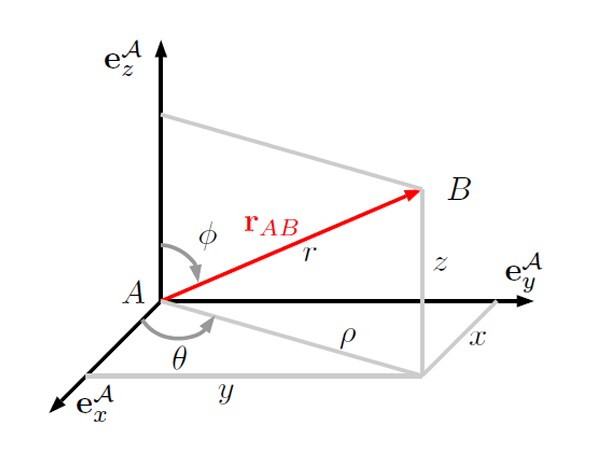
\includegraphics{images/1.jpg}
    \caption{ 使用笛卡尔、柱坐标和球坐标来表示位置}
    \label{label1}
\end{figure}

\begin{equation}
    \left.\mathcal{A}\mathbf{r}=\left(\begin{array}{c}r\cos\theta\sin\phi\\r\sin\theta\sin\phi\\r\cos\phi\end{array}\right.\right)
\end{equation}




\subsection{线速度}


\subsubsection{相对速度}
点 B 相对于点 A 的速度为:

\begin{equation}
    \dot{r}_{AB}
\end{equation}

这里加点表示对时间的导数。

在三维空间中,速度由向量 $\dot{r}\in \mathbb{R}^3$ 表示。

\subsubsection{线速度的表示}
$\chi_{P}$ 表示位置的堆积参数。即,在笛卡尔坐标系下
$$
\left.\chi_{P_c}=\left(\begin{array}{c}x\\y\\z\end{array}\right.\right)
$$
在柱坐标系下
$$
\left.\chi_{P_z}=\left(\begin{array}{c}\rho\\\theta\\z\end{array}\right.\right)
$$
在球坐标系下
$$
\left.\chi_{P_s}=\left(\begin{array}{c}r\\\theta\\\phi\end{array}\right.\right)
$$

速度 $\dot{r}$ 和当前形式下位置的导数 $\dot{\chi}_P$ 之间存在线性映射关系 $E_P(\chi)$:

\begin{equation}
    \dot{\mathbf{r}}=\mathbf{E}_{P}\left(\chi_{P}\right)\dot{\chi}_{P}
\end{equation}

\begin{equation}
    \dot{\chi}_{P}=\mathbf{E}_{P}^{-1}\left(\chi_{P}\right)\dot{\mathbf{r}}
\end{equation}

\noindent\textbf{笛卡尔坐标系}

如果采样笛卡尔坐标系,映射关系 $\mathbf{E}_{P}(\chi)$ 只是简单的单位矩阵
\begin{equation}
    \mathbf{E}_{P_c}\left(\boldsymbol{\chi}_{P_c}\right)=\mathbf{E}_{P_c}^{-1}\left(\boldsymbol{\chi}_{P_c}\right)=\mathbb{I}
\end{equation}

\noindent\textbf{柱坐标}
$$
\left.\chi_{P_c}=\left(\begin{array}{c}x\\y\\z\end{array}\right.\right)=\left(\begin{array}{c}\rho\cos\theta\\\rho\sin\theta\\z\end{array}\right)
$$
从而
$$
\dot{\chi}_{P_c}=\left(\begin{array}{c}\dot{x}\\\dot{y}\\\dot{z}\end{array}\right)=\left(\begin{array}{c}\dot{\rho}\cos\theta-\rho\dot{\theta}\sin\theta\\\dot{\rho}\sin\theta+\rho\dot{\theta}\cos\theta\\\dot{z}\end{array}\right)
=\begin{pmatrix}
    \cos\theta & -\rho\sin\theta & 0 \\
    \sin\theta & \rho\cos\theta & 0 \\
    0 & 0 & 1
    \end{pmatrix}\left(\begin{array}{c}\dot{\rho}\\\dot{\theta}\\\dot{z}\end{array}\right)=\mathbf{E}_{P}\left(\chi_{P}\right)
    \dot{\chi}_{Pz}
$$
从而
$$
\mathbf{E}_{P}^{-1}=
\begin{pmatrix}
    cos\theta & sin\theta & 0 \\
    -sin\theta/\rho & cos\theta/\rho & 0 \\
    0 & 0 & 1 \\
\end{pmatrix}
$$

\noindent\textbf{球坐标}

类似地
$$
\dot{\boldsymbol{\chi}}_{P_{c}}=\left(\begin{array}{c}{\dot{x}}\\{\dot{y}}\\{\dot{z}}\end{array}\right)=\left(\begin{array}{c}{\dot{r}\cos\theta\sin\phi-r\dot{\theta}\sin\theta\sin\phi+r\dot{\phi}\cos\theta\cos\phi}\\{\dot{r}\sin\theta\sin\phi+r\dot{\theta}\cos\theta\sin\phi+r\dot{\phi}\sin\theta\cos\phi}\\{\dot{r}\cos\phi-r\dot{\phi}\sin\phi}\end{array}\right) 
$$
从而
$$
\begin{gathered}
    \mathbf{E}_{Ps}= \left(\begin{array}{ccc}\cos\theta\sin\phi&-r\sin\phi\sin\theta&r\cos\phi\cos\theta\\\sin\phi\sin\theta&r\cos\theta\sin\phi&r\cos\phi\sin\theta\\\cos\phi&0&-r\sin\phi\end{array}\right) \\
    \mathbf{E}_{Ps}^{-1}= \left(\begin{array}{ccc}\cos\theta\sin\phi&\sin\phi\sin\theta&\cos\phi\\-\sin\theta/(r\sin\phi)&\cos\theta/(r\sin\phi)&0\\(\cos\phi\cos\theta)/r&(\cos\phi\sin\theta)/r&-\sin\phi/r\end{array}\right) 
\end{gathered}
$$
\end{document}